\newpage
\subsubsection[QuizziPedia::Front-End::ServiceWorker::Views]{QuizziPedia::Front-End::ServiceWorker::Views}
\begin{figure} [ht]
	\centering
	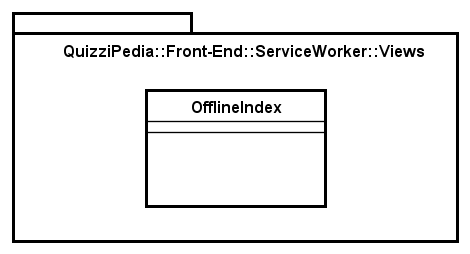
\includegraphics[scale=0.80]{UML/Package/QuizziPedia_Front-End_ServiceWorker_Views.png}
	\caption{QuizziPedia::Front-End::ServiceWorker::Views}
\end{figure} \FloatBarrier

\subsubsection{Informazioni generali}
\begin{itemize}
	\item \textbf{Descrizione}:	;
	\item \textbf{Padre}: \texttt{Front-End};
	\item \textbf{Interazione con altri componenti}:
	\begin{itemize}
		\item \texttt{Directives}: ;
		\item \texttt{Views}: .
	\end{itemize} 
\end{itemize}
\subsubsection{Classi}

\paragraph[QuizziPedia::Front-End::ServiceWorker::Views::OfflineIndex]{QuizziPedia::Front-End::ServiceWorker::Views::OfflineIndex}
\begin{figure} [ht]
	\centering
	\includegraphics[scale=0.80]{UML/Classi/Front-End/QuizziPedia_Front-End_ServiceWorker_Views_OfflineIndex.png}
	\caption{QuizziPedia::Front-End::ServiceWorker::Views::OfflineIndex}
\end{figure} \FloatBarrier
\begin{itemize}
	\item \textbf{Descrizione}: \textit{view\ped{G}} generale dell'applicazione offline;
	\item \textbf{Utilizzo}: contiene gli elementi che saranno presenti nella pagina dell'applicazione offline.
\end{itemize}



